\section{Software Architecture and Implementation}

The software is organized as two cooperating parts: ESP-IDF firmware running on the
ESP32 and a browser-based control interface. The firmware owns the real-time work:
GPIO switching, analog acquisition, BLE services, and command execution. The web
application is intentionally thin: it connects through Web Bluetooth, sends commands,
and plots the status and measured voltages returned by the ESP32.

This separation is important for reproducibility. A reader implementing the system
should keep all timing-critical decisions inside the firmware and use the browser only
as a user interface. The browser may pause, render slowly, or lose focus; the ESP32
must continue to generate the selected switching pattern without depending on those
events.

\subsection{Firmware Task Organization}

The firmware starts by configuring the output GPIOs, ADC channels, non-volatile
storage, BLE services, and the default modulation pattern. After initialization, the
main runtime is divided into three functional paths:

\begin{itemize}
	\item \textbf{Signal generation:} a high-priority task pinned to Core 1 writes the
	      six switch-control GPIOs using precomputed register masks.
	\item \textbf{Communication and commands:} BLE handling and UI command dispatch run
	      on Core 0, where timing jitter does not directly affect the switching loop.
	\item \textbf{Analog monitoring:} a background acquisition task samples AN3, AN5,
	      and AN6, calibrates the readings, and publishes coherent snapshots for
	      telemetry and optional closed-loop correction.
\end{itemize}

The ESP32 is configured to run at 240 MHz, so one microsecond corresponds to 240 CPU
cycles. The signal task uses this fixed conversion to schedule sub-microsecond
dead-time and microsecond-scale segment durations. Core 1's idle-task watchdog check is
disabled because the signal loop may intentionally occupy the core during continuous
waveform generation.

\begin{table}[htbp]
	\centering
	\caption{Firmware configuration relevant to reproduction}
	\label{tab:system-config}
	\begin{tabular}{llp{7.6cm}}
		\toprule
		\textbf{Item} & \textbf{Value} & \textbf{Purpose} \\
		\midrule
		CPU frequency & 240 MHz & Defines the cycle-to-time conversion used by the signal loop. \\
		Signal task core & Core 1 & Isolates GPIO timing from BLE and browser-originated commands. \\
		BLE and command core & Core 0 & Keeps parsing, logging, and notifications outside the hot path. \\
		Signal buffers & Two & Allows one active pattern and one inactive pattern being updated. \\
		ADC inputs & AN3, AN5, AN6 & Measures the converter feedback voltages used for monitoring. \\
		\bottomrule
	\end{tabular}
\end{table}

\subsection{Signal Pattern Pipeline}

The switching waveform is represented by two vectors: segment duration in
microseconds and segment mode. The mode is the decimal encoding of three binary
control signals, later expanded into the six complementary gate commands. For example,
mode 5 corresponds to the binary state 101 for the three logical switch variables.

New patterns are never written into the active buffer. When a command such as
\verb|signal.set_pattern| or \verb|signal.set_alpha| arrives, the firmware selects the
inactive dataset, fills the raw duration and mode arrays, expands each mode into
individual switch states, and precomputes the GPIO masks required by the signal loop.
Only after this preparation is complete does it set the update-pending flag.

\begin{lstlisting}[caption={Updating the inactive signal buffer}, label={lst:inactive-buffer}]
if (g_active_set == SignalSet::SET_A) {
    target_dataset = &g_dataset_b;
} else {
    target_dataset = &g_dataset_a;
}

parse_signal(message, times, modes);
// Fill time_durations[] and modes_d4/d5/d6[] here.
signal_precompute_steps(target_dataset);
g_ds_update_pending = true;
\end{lstlisting}

The running task checks this flag only between complete pattern cycles. The pointer
swap is therefore atomic from the viewpoint of the generated waveform: the output
never uses half of an old pattern and half of a new one.

\begin{lstlisting}[caption={Cycle-boundary buffer swap}, label={lst:buffer-swap}]
if (g_ds_update_pending.load(std::memory_order_acquire)) {
    if (g_active_set.load() == SignalSet::SET_A) {
        ctx.dataset = &g_dataset_b;
        g_active_set.store(SignalSet::SET_B);
    } else {
        ctx.dataset = &g_dataset_a;
        g_active_set.store(SignalSet::SET_A);
    }
    g_ds_update_pending.store(false, std::memory_order_release);
}
\end{lstlisting}

\subsection{GPIO Timing Loop}

The critical optimization is to move computation out of the playback loop. Each
\verb|SignalStep| stores the masks to clear, the masks to set, the dead-time in CPU
cycles, and the segment duration already converted to cycles. During playback, the
loop only waits for the next edge, applies dead-time when a leg changes state, and
writes the GPIO registers.

\begin{lstlisting}[caption={Precomputed step used by the playback loop}, label={lst:signal-step}]
struct SignalStep {
    uint32_t set_mask;         // GPIO.out_w1ts
    uint32_t clr_mask;         // GPIO.out_w1tc
    uint32_t clear_mask;       // both devices off before transition
    uint32_t dead_time;        // CPU cycles
    uint32_t duration_cycles;  // segment duration
};
\end{lstlisting}

The firmware uses the ESP32 write-one-to-set and write-one-to-clear GPIO registers.
In the code these are \verb|GPIO.out_w1ts| and \verb|GPIO.out_w1tc|. They update
multiple pins with one write, avoiding the skew that would appear if each output were
changed by separate high-level GPIO calls.

\begin{lstlisting}[caption={Atomic GPIO transition with dead-time}, label={lst:switching}]
if (step.clear_mask) {
    GPIO.out_w1tc = step.clear_mask;
    helper_delay_cycles(step.dead_time);
}

GPIO.out_w1tc = step.clr_mask;
GPIO.out_w1ts = step.set_mask;
\end{lstlisting}

This approach is the main implementation rule for reproducing the firmware: parse and
validate outside the loop, precompute all masks and durations, and reserve the
interrupt-disabled section for register writes and exact waits only.

\subsection{Analog Acquisition and Calibration}

The firmware measures three feedback voltages through ADC1 channels mapped to AN3,
AN5, and AN6. The ADC path supports one-shot acquisition and continuous DMA
acquisition. Continuous mode is used when fresh feedback is required at higher rate;
the DMA samples are regrouped into complete AN3/AN5/AN6 triples before publication.

Raw ADC codes are converted to voltage and then corrected with a calibration lookup
table. The table is generated at startup from measured calibration points using linear
interpolation, so runtime conversion is a simple indexed lookup in the acquisition
path.

\begin{lstlisting}[caption={Runtime ADC calibration lookup}, label={lst:calib}]
float analog_calibrate_raw_lut(uint32_t raw) {
    if (raw > ANALOG_ADC_MAX_CODE) {
        raw = ANALOG_ADC_MAX_CODE;
    }
    if (!s_calibration_lut_ready.load()) {
        return analog_calibrate_raw(raw);
    }
    return s_calibration_lut[raw];
}
\end{lstlisting}

Each valid sample triple is stored as a coherent snapshot with a sequence counter. The
signal loop can reject stale samples, while the BLE telemetry task can read the latest
calibrated values without blocking the ADC task.

\subsection{BLE Protocol and Web Interface}

The BLE protocol uses two message styles. Human-readable UI commands are sent as a
command name plus a small JSON payload. Firmware responses, status packets, diagnostic
results, and voltage telemetry are encoded with Protocol Buffers to keep the BLE
payload compact and typed.

\begin{table}[htbp]
	\centering
	\caption{Main browser-to-firmware commands}
	\label{tab:ble-commands}
	\begin{tabular}{llp{7.4cm}}
		\toprule
		\textbf{Command} & \textbf{Payload} & \textbf{Effect} \\
		\midrule
		\verb|signal.start| & \verb|{}| & Starts the Core 1 signal task. \\
		\verb|signal.stop| & \verb|{}| & Stops the signal task and forces all switch outputs low. \\
		\verb|signal.set_alpha| & \verb|{"alpha":x}| & Computes the phase-shift modulation pattern for duty parameter $x$. \\
		\verb|signal.set_pattern| & \verb|{"time":"...","mode":"..."}| & Uploads explicit duration and mode vectors to the inactive buffer. \\
		\verb|signal.set_dead_time| & \verb|{"time_us":x}| & Updates the compensated dead-time used in future precomputed steps. \\
		\verb|analog.read_once| & \verb|{}| & Sends one calibrated analog reading packet. \\
		\verb|system.get_status| & \verb|{}| & Sends signal, BLE, analog, and timing status. \\
		\bottomrule
	\end{tabular}
\end{table}

The web interface shown in Fig. \ref{fig:sw_web_interface} implements this command
layer in the browser. It scans for the ESP32 BLE service, connects to its GATT
characteristic, writes UI commands, decodes protobuf notifications, and plots the
received analog values. No native driver is required, which makes the setup easier to
repeat on a laboratory computer.

\begin{figure}[h!]
	\centering
	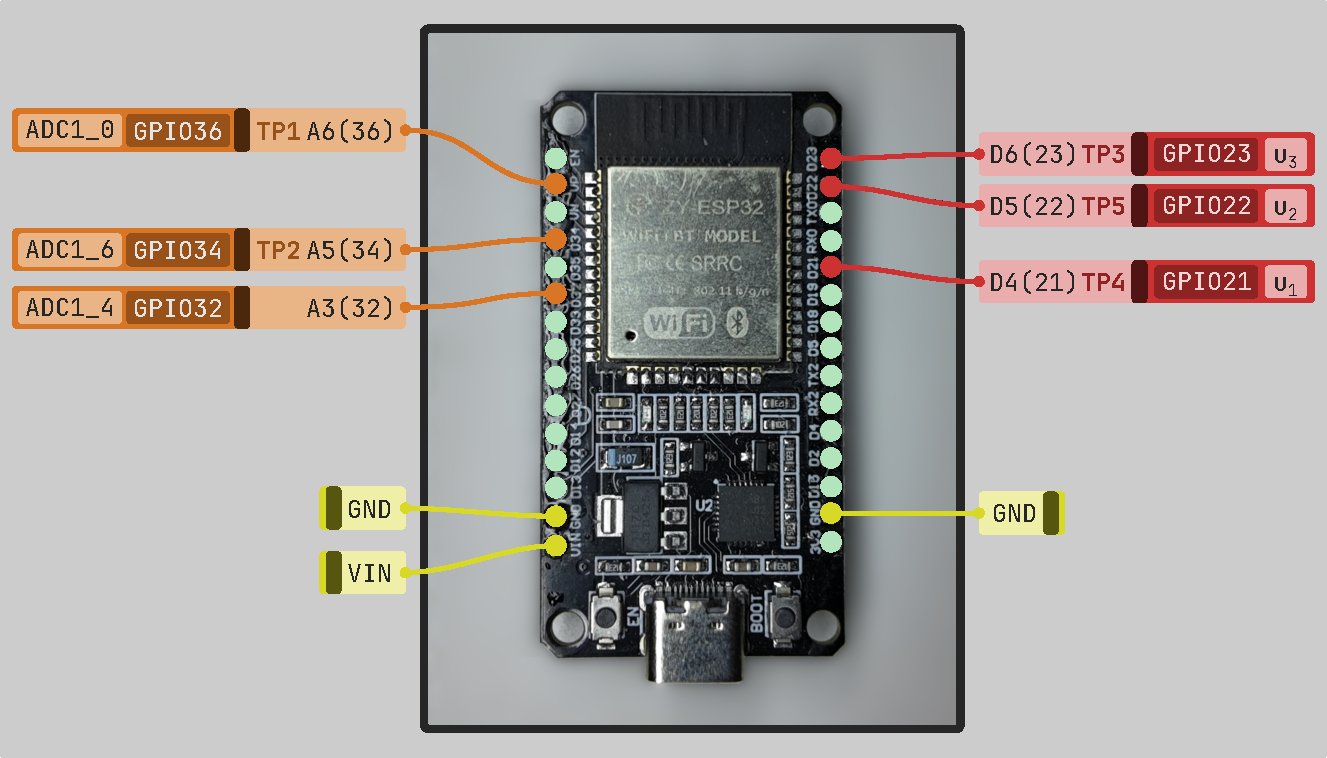
\includegraphics[width=140mm]{figures/images/hw_esp32_pins.pdf}
	\caption{ESP32 digital output and analog input mapping used by the firmware.}
	\label{fig:sw_esp_pins}
\end{figure}

\begin{figure}[h!]
	\centering
	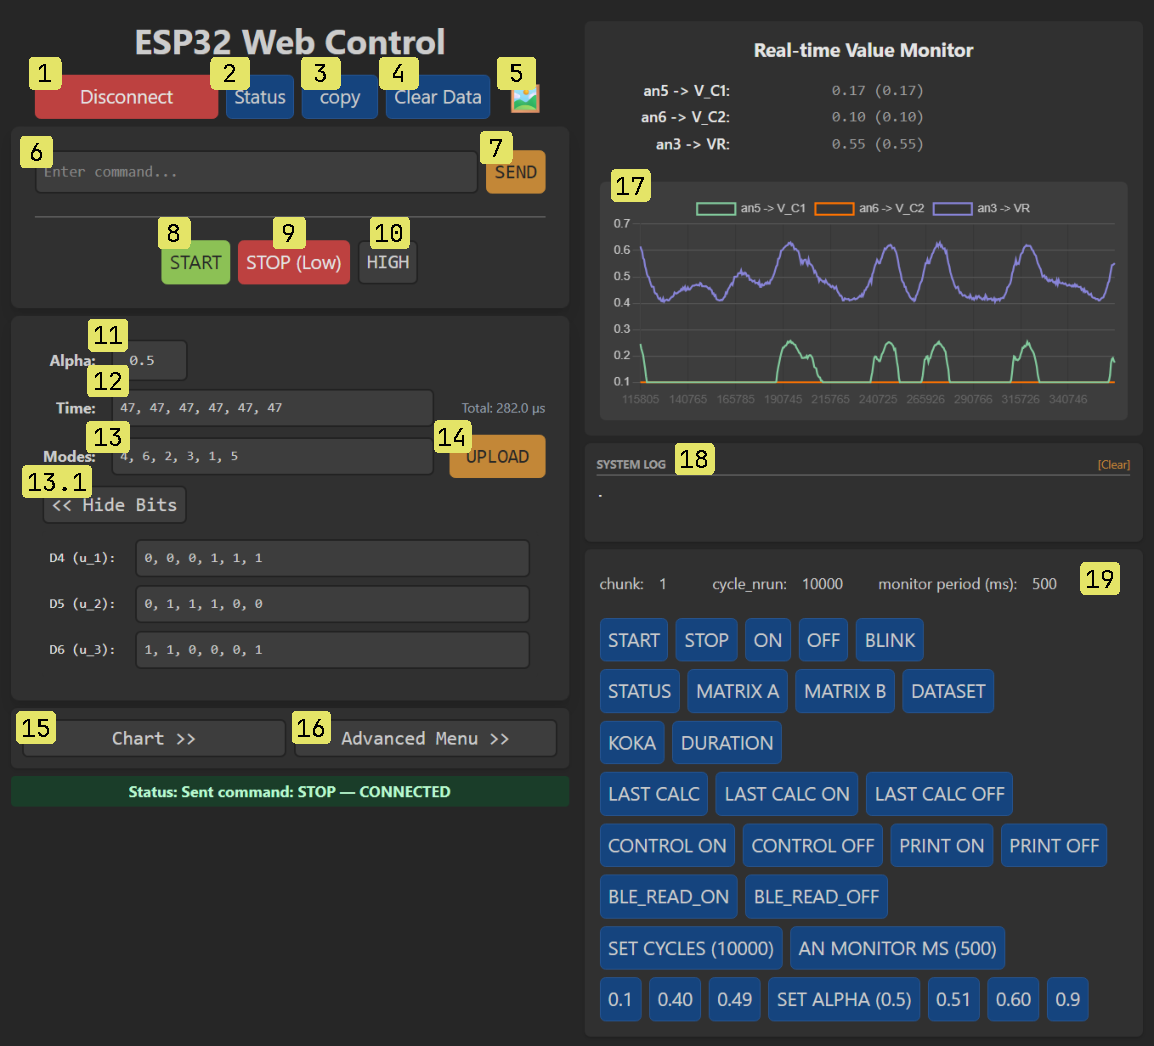
\includegraphics[width=140mm]{figures/images/sw_web_interface.pdf}
	\caption{Browser interface for BLE connection, signal upload, and telemetry plotting.}
	\label{fig:sw_web_interface}
\end{figure}

\begin{figure}[h!]
	\centering
	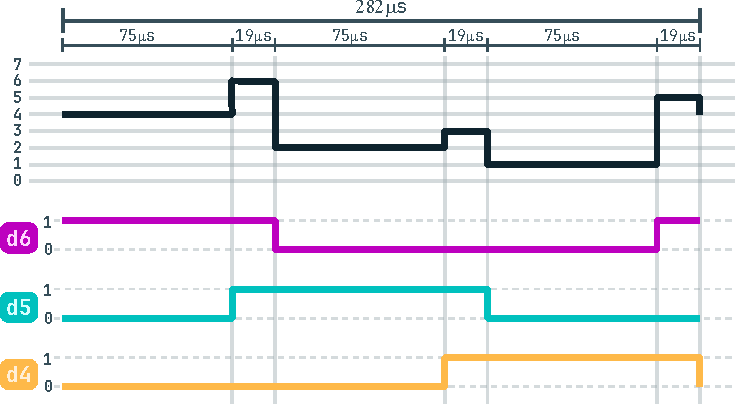
\includegraphics[width=140mm]{figures/images/sw_signal.pdf}
	\caption{Example digital switching pattern generated from the phase-shift parameter.}
	\label{fig:sw_signal}
\end{figure}

Figure \ref{fig:state_diagram} summarizes the firmware states. The communication path
may be idle, reading analog data, or processing commands while the signal path is
independently stopped or running. This state separation is what allows the experimenter
to update parameters and inspect telemetry without inserting browser-dependent timing
into the switching loop.

\begin{figure}[h]
	\centering
	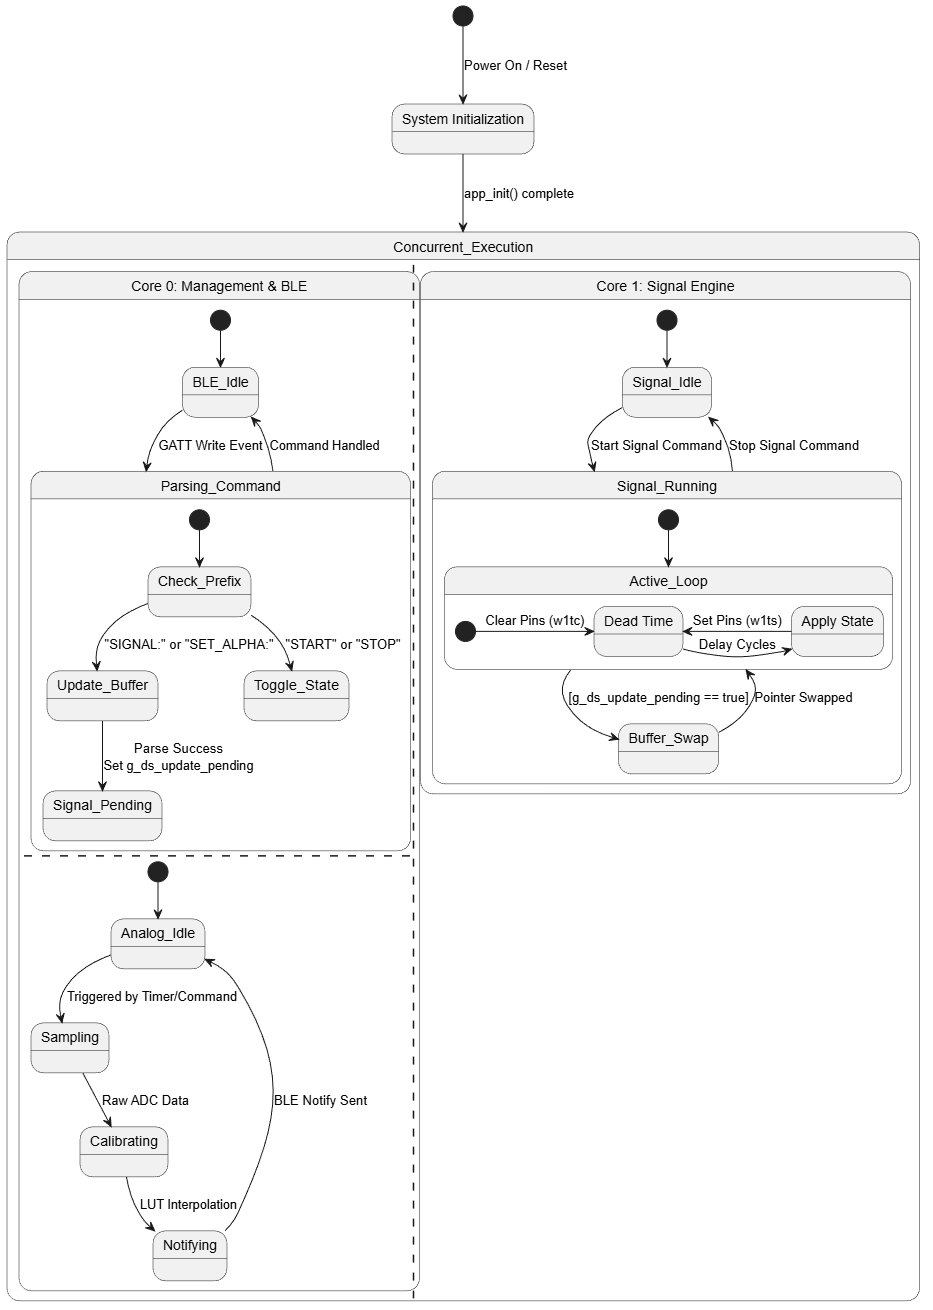
\includegraphics[scale=0.5]{figures/images/sw_state_machine.png}
	\caption{Firmware operation states for BLE, analog acquisition, and signal generation.}
	\label{fig:state_diagram}
\end{figure}
